\section{Evaluation} \label{sec:evaluation}

\subsection{Qualitative grading with LLM judge} \label{sec:qualitative-llm-judge}

Adopting best practices from \citet{guSurveyLLMasaJudge2025}, we

We also calculated whether the difference in scores was statistically significant using (1) a Wilconoxon signed-rank test for Likert ratings with paired samples and (2) a binomial test for boolean ratings. We set the significance level at 0.05.


\begin{figure}[htb]
  \centering
  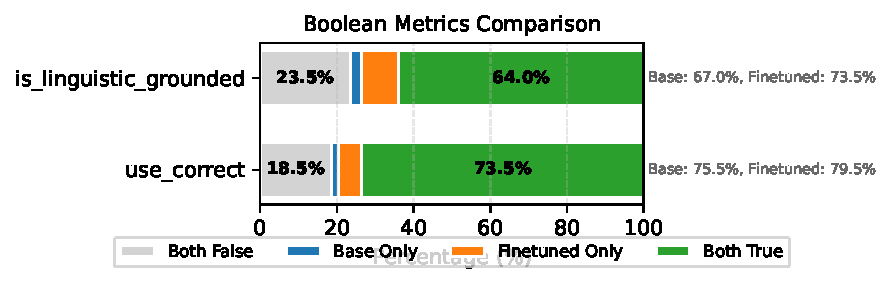
\includegraphics[width=\linewidth]{figures/boolean_comparison.pdf}
  \caption{LLM-as-a-judge for boolean ratings. FILL IN RESULTS HERE}
  \label{fig:llm-judge-boolean}
\end{figure}

\begin{figure}[htb]
  \centering
  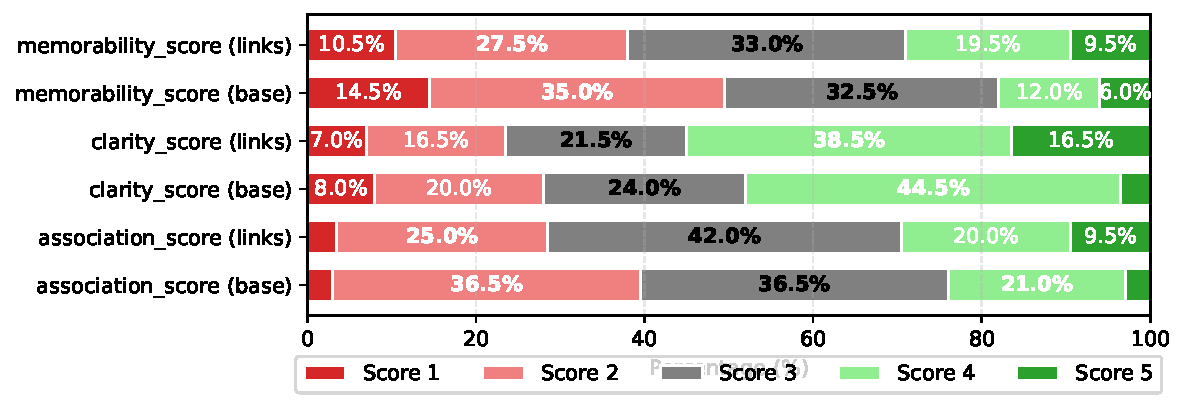
\includegraphics[width=\linewidth]{figures/likert_distribution.pdf}
  \caption{LLM-as-a-judge for 1-5 Likert ratings. FILL IN WHAT THE SCORES MEAN AND RESULTS HERE}
  \label{fig:llm-judge-likert}
\end{figure}

\subsection{Pairwise preference using double-blind annotations} \label{sec:pairwise-preference}
We conducted a double-blind annotation study to evaluate the quality of mnemonics generated by different methods. We randomly selected 50 mnemonics from each method and presented them to annotators in pairs, asking them to choose the better mnemonic for each pair. This approach allowed us to obtain a more nuanced understanding of the relative performance of each method. In the interest of time, we only used two annotators (the author and a different LLM, \judgemodel), and noted this as a limitation in \Cref{sec:limitations}. The annotators were instructed to consider the following criteria when making their judgments:

\begin{figure}[htb]
  \centering
  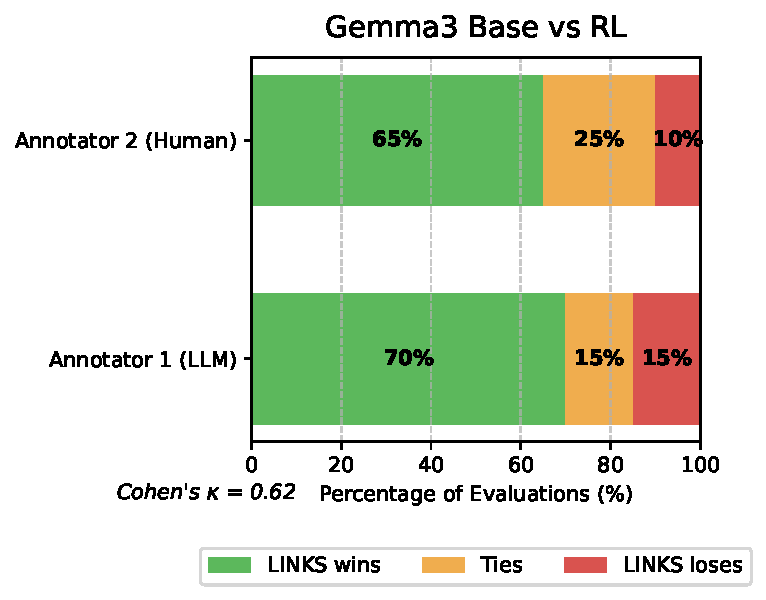
\includegraphics[width=\linewidth]{figures/model_comparison.pdf}
  \caption{Pairwise preference using double-blind annotation. Y-axis shows the percentage of preference for each mnemonic generation method.}
\end{figure}
